\documentclass[titlepage, 12pt]{article}
\usepackage[parfill]{parskip}
\usepackage{xcolor}
\usepackage{setspace}
\usepackage{hyperref}
\usepackage[T1]{fontenc}
\usepackage[utf8]{inputenc}
\usepackage{graphicx}
\usepackage{microtype}
\graphicspath{ {./assets/} }

\usepackage{charter}

\hypersetup{
    colorlinks=true,
    linkcolor=blue,
    filecolor=magenta,
    urlcolor=blue,
}

\begin{document}

\begin{titlepage}

	\raggedleft

	\vspace*{\baselineskip}

	{Bharathi Ramana Joshi 2019121006\\Jayati Narang 2018101066}

	\vspace*{0.167\textheight}

	\textbf{\Large Report for}\\[\baselineskip]

	\textbf{\textcolor{teal}{\huge Data visualization}}\\[\baselineskip]

    {\large \textit{Team: namesarehard}}
    \vfill

    \today

	\raggedright

\end{titlepage}

\newpage

\tableofcontents

\newpage

\section{Essential Links}
\subsection{Demo Video}
\subsection{Dataset used} The dataset that we used is \href{https://www.kaggle.com/uciml/student-alcohol-consumption/data}{Student Alcohol Consumption}. 
\subsection{Purpose of the data visualisation}
We used this to not only analyse students' alcohol consumption pattern but also to examine various factors which affect students' study, for example, family support, extra educational support, parents education and job etc. We tried to answer a plethora of questions using this dataset.
Some of the relationships we tried to establish are :
\begin{itemize}
    \item How does family support depend on the parent's education?
    \item What's the association between the parent's education and job status?
    \item How does a student's alcohol consumption level related to his relationship status?
    \item How family's support can affect a student's drinking habit?
    \item How to relate grades with study time?

\end{itemize}
\subsection{Analysis from the visualisation}
 
\subsubsection{Parents' education and employment vs support}

\begin{center}
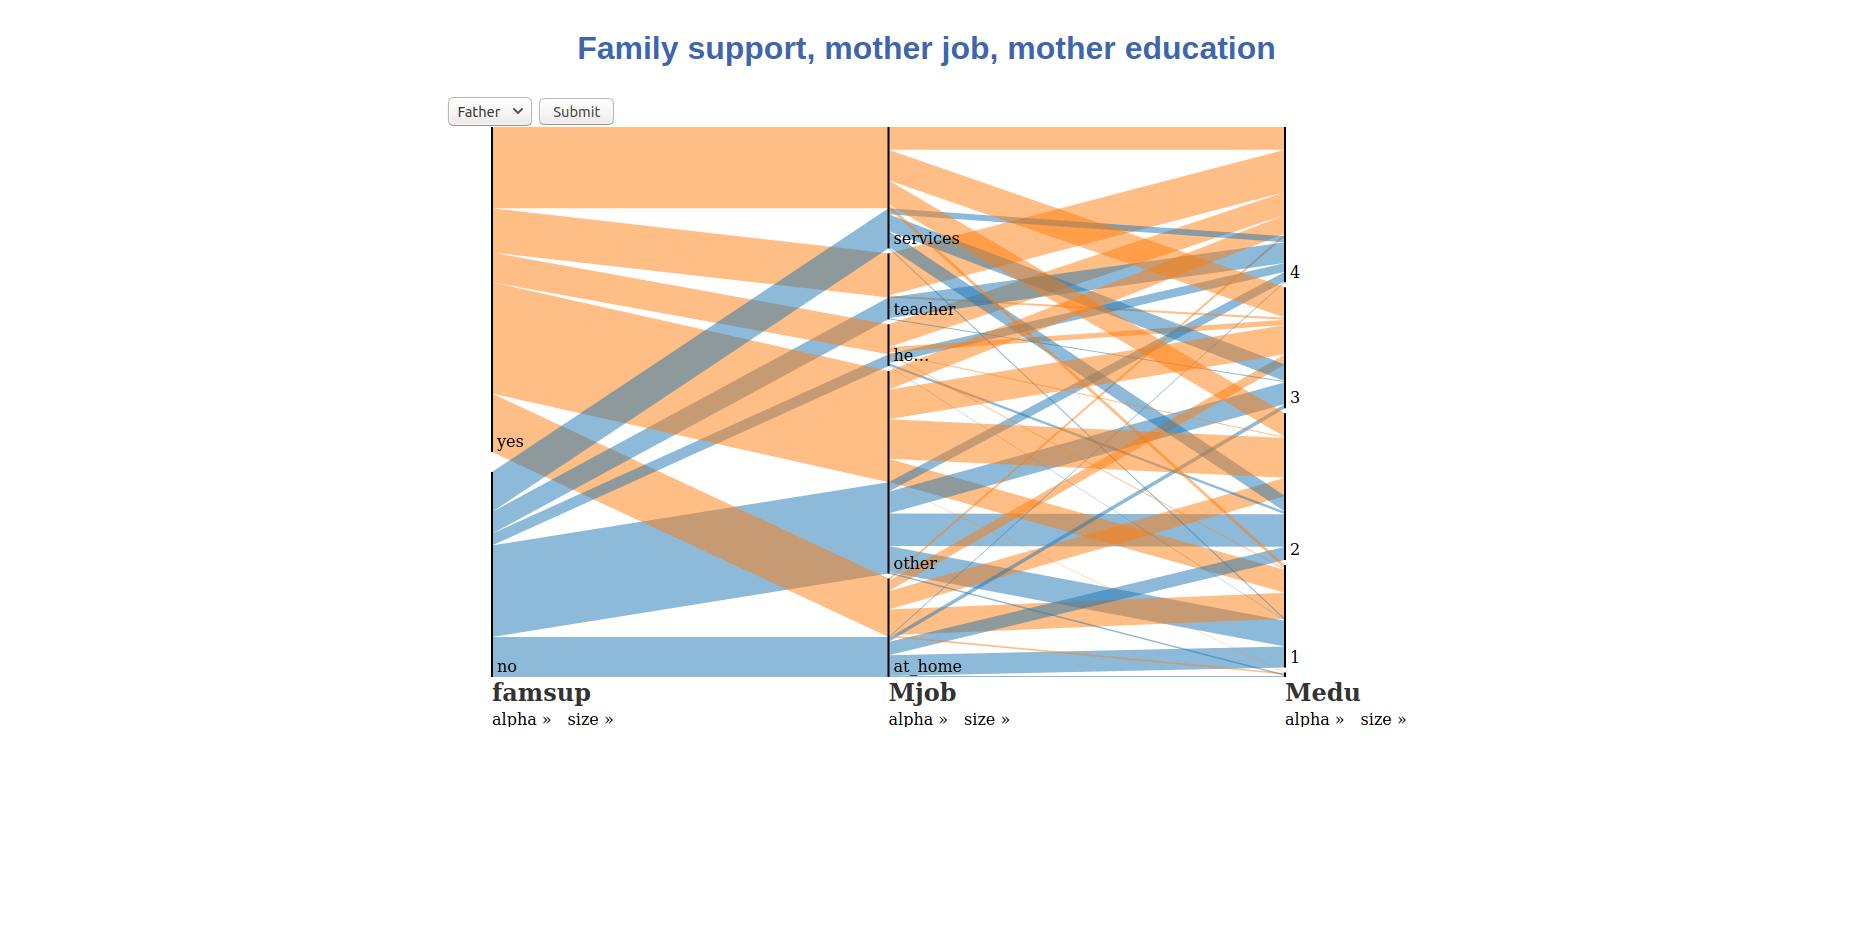
\includegraphics[scale=0.2]{1}
\end{center}
\begin{itemize}
    \item Irrespective of the level of a parent’s education, the portion of families supporting children’s education is more than the portion not supporting it i.e. families are, in most cases, supportive of children’s education irrespective of parent’s education.
    \item Higher levels of parent’s education leads to higher job status.
\end{itemize}


\subsubsection{Binary field vs Alcohol consumption}
\begin{center}
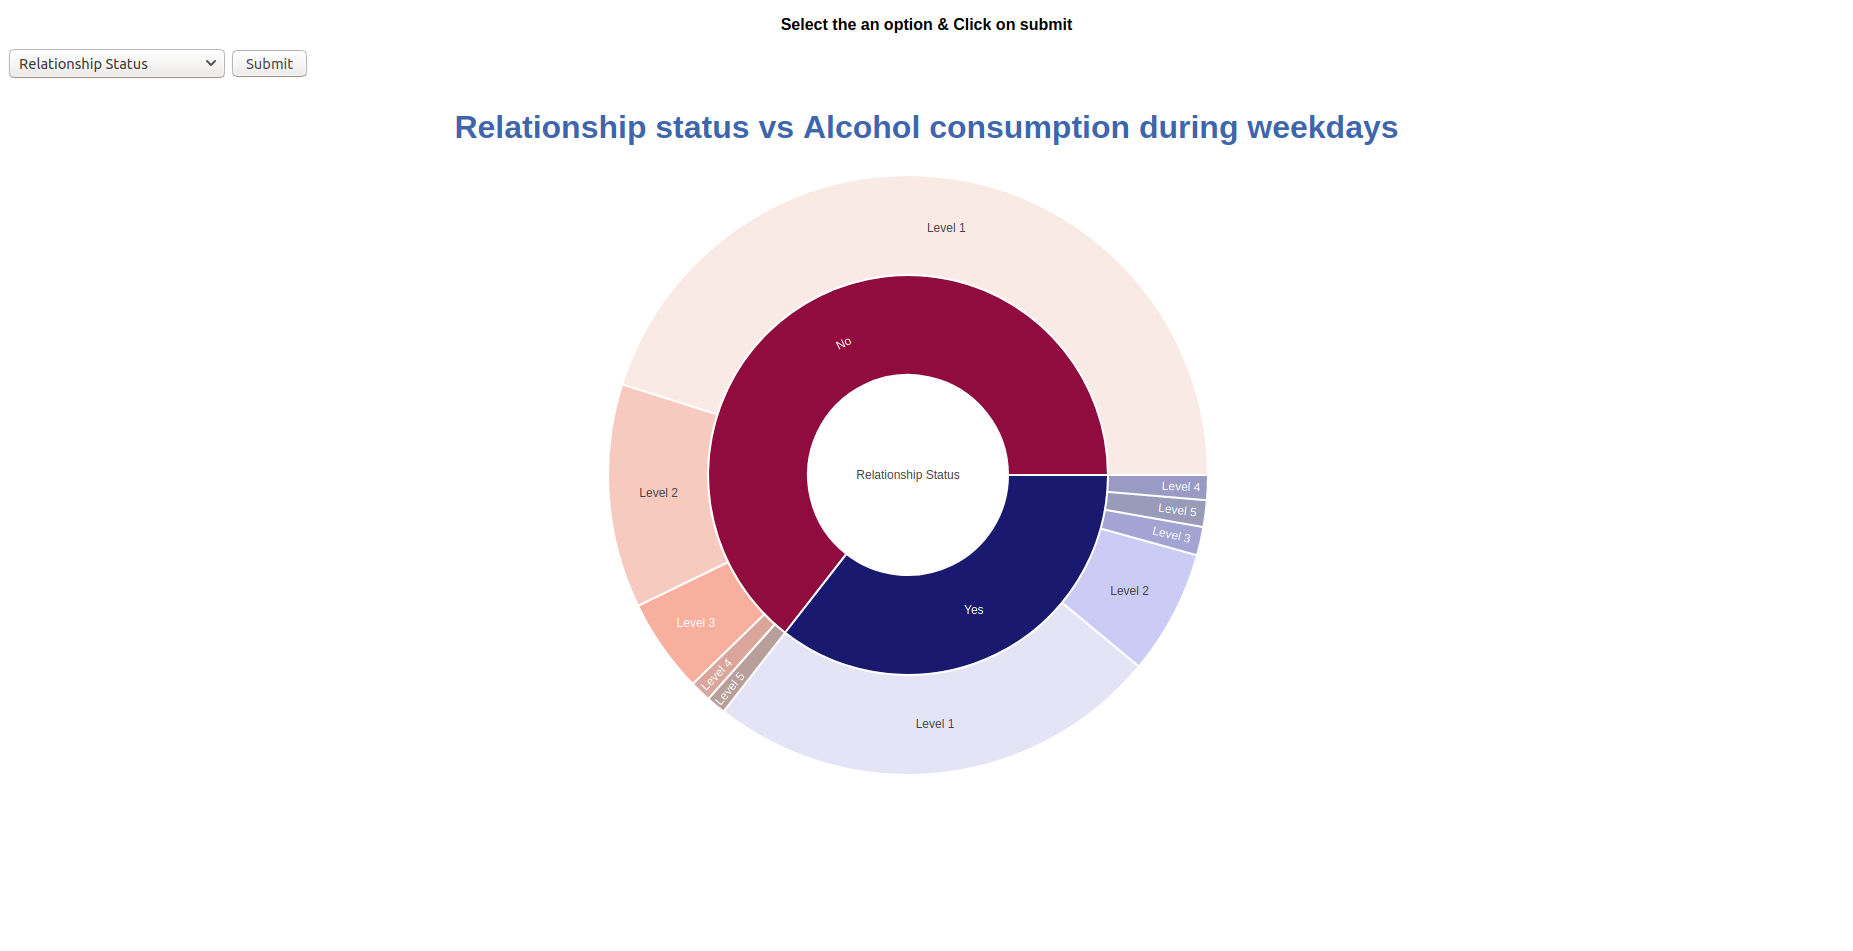
\includegraphics[scale=0.2]{2}
\end{center}
\begin{itemize}
    \item Irrespective of relationship status, level of alcohol consumption is inversely proportional to the population i.e. higher the level of consumption, lesser the number of students consuming alcohol at that level.
    \item As the level of consumption increases, males tend to drink more than females. Ironically, students with family support tend to drink more.
    \item As expected, students without extra school support tend to drink more than those with it.
\end{itemize}
\subsubsection{Study time vs grades}
For any given study time, the students’ grades are roughly distributed over a bell curve
Higher the study time of a student, more likely they are to get a good grade
\begin{center}
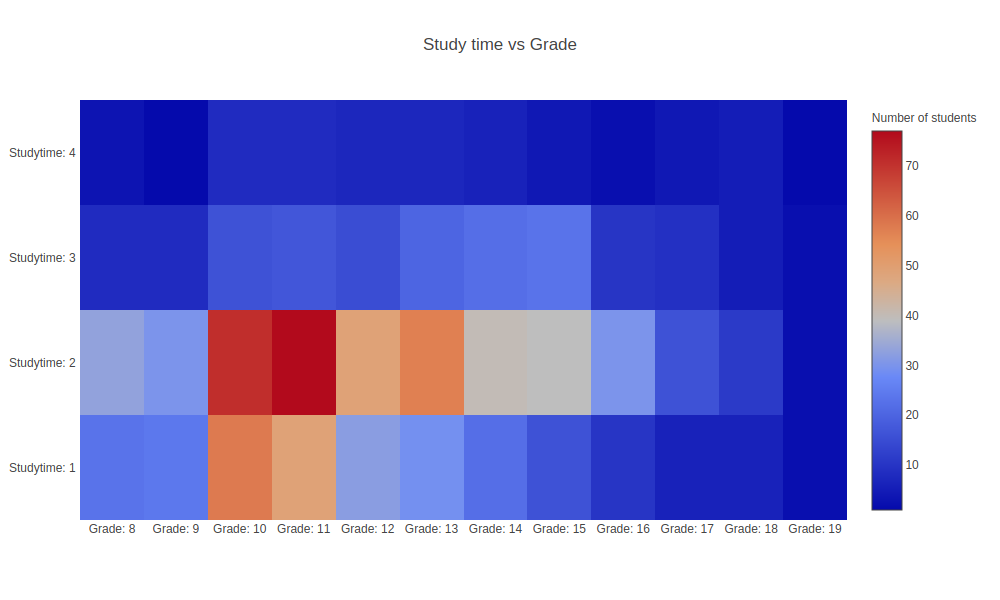
\includegraphics[scale=0.3]{3}
\end{center}

\subsubsection{Absences, parents' habitation status vs avg.failures}
\begin{center}
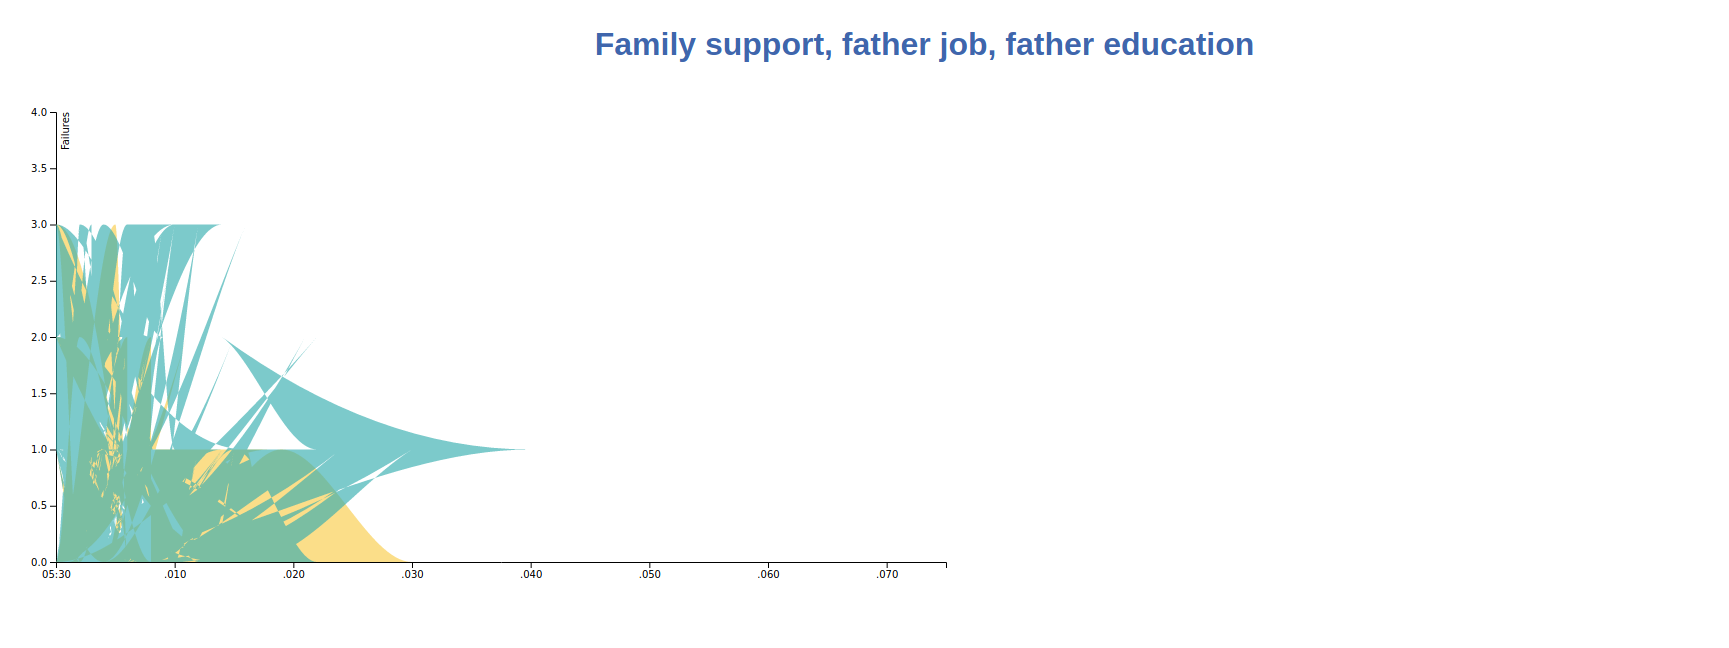
\includegraphics[scale=0.2]{5}
\end{center}
\subsubsection{Family size, relationships' quality vs alcohol consumption}
\begin{center}
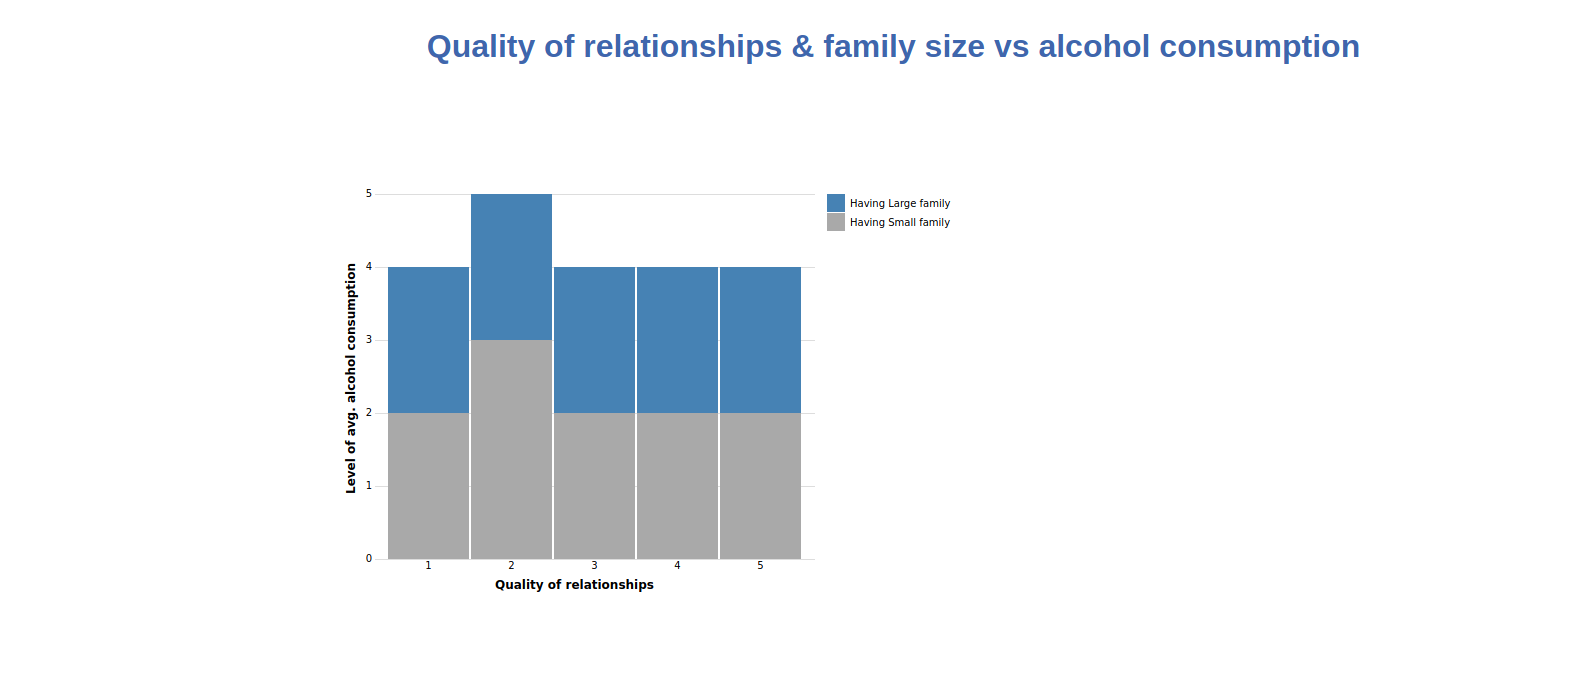
\includegraphics[scale=0.2]{8}
\end{center}




\section{Conclusion}

\end{document}
